\documentclass{beamer}

\usepackage[utf8]{inputenc} % Language and font encoding
\usepackage[icelandic]{babel}
\usepackage[T1]{fontenc}


\usepackage{tikz}
\usepackage[listings,theorems]{tcolorbox}
\usepackage{booktabs}
\usepackage{minted} %Minted and configuration
\usemintedstyle{default}

\renewcommand{\theFancyVerbLine}{\sffamily \arabic{FancyVerbLine}}
%%%%%%%%%%%
% More math
%%%%%%%%%%%
\newcommand{\Mod}[1]{\ \text{mod}\ #1}

%%%%%%%%%%%%%%%%%%%%%%
% Beamer configuration
%%%%%%%%%%%%%%%%%%%%%%
\setbeamertemplate{navigation symbols}{}
\usecolortheme{dove}
\setbeamercolor{frametitle}{fg=white}

\usebackgroundtemplate%
{%
\vbox to \paperheight{

\includegraphics[width=\paperwidth]{Pics/hi-slide-head-2016}

\vfill
\hspace{0.5cm}
\includegraphics[width=0.3\paperwidth]{Pics/hi-von-logo}
\vspace{0.4cm}
    }%
}

\AtBeginSection[]
{
  \begin{frame}<beamer>
    \frametitle{Yfirlit}
    \tableofcontents[currentsection]
  \end{frame}
}

\setbeamerfont{frametitle}{size=\normalsize}
\addtobeamertemplate{frametitle}{}{\vspace*{0.5cm}}

%%%%%%%%%%%%%%%%%%%%%%%%%
% tcolorbox configuration
%%%%%%%%%%%%%%%%%%%%%%%%%

% Setup from: http://tex.stackexchange.com/a/43329/21638
\tcbset{%
    noparskip,
    colback=gray!10, %background color of the box
    colframe=gray!40, %color of frame and title background
    coltext=black, %color of body text
    coltitle=black, %color of title text 
    fonttitle=\bfseries,
    alerted/.style={coltitle=red, colframe=gray!40},
    example/.style={coltitle=black, colframe=green!20, colback=green!5},
}


%%%%%%%%%%%%%%%%%%%%%%%
% Further configuration
%%%%%%%%%%%%%%%%%%%%%%%
\hypersetup{colorlinks=true,pdfauthor={Eirikur Ernir Thorsteinsson},linkcolor=blue,urlcolor=blue}
\graphicspath{{./Pics/}}

\author{Eiríkur Ernir Þorsteinsson}
\institute{Háskóli Íslands}
\date{Haust 2016}

\title{Stærðfræðimynstur í tölvunarfræði}
\subtitle{Vika 3, fyrri fyrirlestur}

\begin{document}

\begin{frame}
\titlepage
\end{frame}

\section{Inngangur}

\begin{frame}{Í síðasta tíma}
\begin{itemize}
 \item Föll
 \item Fylki
 \item Runur og rakningarvensl
 \item Fjöldatölur og reiknanleiki
\end{itemize}
\end{frame}

\section{Skilgreining reiknirits}

\begin{frame}{Vandamál í tölvunarfræði}
\begin{itemize}
 \item Tölvunarfræði felur í sér ýmis vandamál, sum þeirra koma oft fyrir
 \begin{itemize}
  \item Finnum stærstu töluna í þessari runu heiltalna
  \item Tökum þessa runu heiltalna og endurröðum henni í hækkandi röð
  \item Finnum stystu leið á milli þessara tveggja hnúta í neti
 \end{itemize}
 \item Til að tákna vandamálin notum við mengi, runur, föll, net, tré, endanlegar stöðuvélar\ldots
 \item Til að leysa vandamálin notum við \emph{reiknirit}
\end{itemize}
\end{frame}

\begin{frame}{Reiknirit}
Hvað er reiknirit? \pause

Úr bók:
\begin{tcolorbox}[title=Reiknirit]
Reiknirit (e. \emph{algorithm}) er endanleg runa vel skilgreindra aðgerða sem reikna út niðurstöðu á skilgreindu vandamáli.
\end{tcolorbox}

Orðið ``algorithm'' er afleiða latneskunar á nafinu al-Khowarizmi, sem skrifaði um hindú-arabíska talnakerfið. Bók hans, \emph{Kitab al-jabr w'al muquabala}, er þekkt grundvallarrit.

\pause
Orðið kemur fram í \href{https://en.wikipedia.org/wiki/Hauksb\%C3\%B3k}{Hauksbók}!
\end{frame}

\section{Lýsing og eiginleikar reiknirita}

\begin{frame}{Eiginleikar reiknirita}
\begin{itemize}
 \item Nokkrir eiginleikar eru flestum reikniritum sameiginlegir
 \item Koma fyrir aftur og aftur í lýsingum reiknirita
 \begin{itemize}
  \item Vandamál sem leysa skal
  \item Inntak (e. \emph{input})
  \begin{itemize}
   \item Reiknirit tekur við gildum úr skilgreindu mengi, gildin eru inntak þess
   \item Inntak reiknirits inniheldur upplýsingar sem viðkoma vandamálinu
  \end{itemize}
  \item Úttak (e. \emph{output})
  \begin{itemize}
   \item Úttak reiknirits tilheyrir skilgreindu mengi
   \item Úttakið lýsir niðurstöðum reikniritsins, sem er lausn á vandamáli
  \end{itemize}
 \end{itemize}
\end{itemize}
\end{frame}

\begin{frame}{Fleiri atriði í reikniritalýsingum}
\begin{itemize}
 \item Fleiri atriði:
 \begin{itemize}
  \item Sé hvert skref reiknirits vel skilgreint og ákvarðanlegt er það skýrt (e. \emph{definite})
  \item Skili reiknirit væntri niðurstöðu fyrir sérhvert inntak er það rétt (e. \emph{correct})
  \item Skili reiknirit niðurstöðu á endanlegum tíma er það endanlegt (e. \emph{finite})
  \item Virki reiknirit á öll tilvik vandamálsins er það almennt (e. \emph{general})
 \end{itemize}
 \item Oftast viljum við að reiknirit hafi alla þessa eiginleika
\end{itemize}
\end{frame}

\begin{frame}{Lýsing reiknirita}
Hægt er að nota orð til að lýsa reikniritum. Dæmi úr bók til að finna stærstu heiltölu í runu:

\begin{enumerate}
 \item Set the temporary maximum equal to the first integer in the sequence.
 \item Compare the next integer in the sequence to the temporary maximum, and if it is larger
than the temporary maximum, set the temporary maximum equal to this integer.
 \item Repeat the previous step if there are more integers in the sequence.
 \item Stop when there are no integers left in the sequence. The temporary maximum at this
point is the largest integer in the sequence.
\end{enumerate}
\end{frame}

\begin{frame}{Sauðakóði}
\begin{columns}
\column{0.6\textwidth}
\begin{itemize}
 \item Orðalýsing á reikniritum er oft mjög löng og óþægileg
 \item Til að auðvelda lýsingar nota ýmsir höfundar oft svokallaðan sauðakóða (e. \emph{pseudocode})
 \item Sauðakóði á að vera ``auðveldur aflestrar''
 \begin{itemize}
  \item Í sauðakóða vantar ýmis útfærsluatriði sem algeng eru í forritunarmálum
  \item Í sauðakóða er leyfilegt að lýsa atriðum sem myndu taka margar aðgerðir í tölvu með því að nota setningar
 \end{itemize}
\end{itemize}
\column{0.4\textwidth}
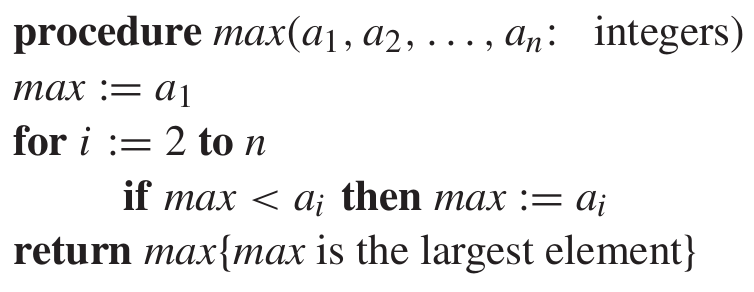
\includegraphics[width=\linewidth]{max-element}

Reiknirit til að finna stærstu heiltölu í runu heiltalna.
\end{columns}
\end{frame}

\begin{frame}{Rétt reiknirit}
\begin{columns}
\column{0.5\textwidth}
Hægt er að nota fastayrðingar\\
(e. \emph{invariants}) til að sanna réttleika forrita
\column{0.5\textwidth}
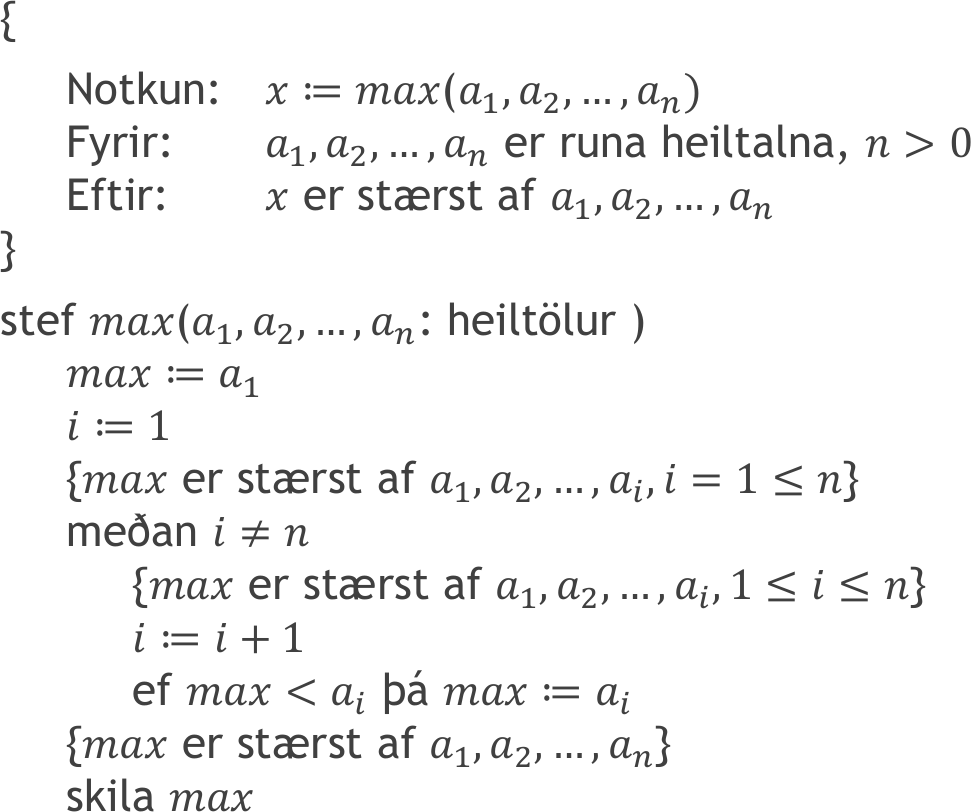
\includegraphics[width=\linewidth]{invariants}
\end{columns}
\end{frame}

\section{Leitarreiknirit}

\begin{frame}{Leitarreiknirit}
\begin{itemize}
 \item Leit að lið í runu kemur víða við
 \begin{itemize}
  \item Er þessi nemandi í námskeiðinu? 
  \item Er þetta orð rétt skrifað?
 \end{itemize}
 \item Getum skilgreint leitarvandamálið fyrir runur:
 \begin{itemize}
  \item Gefið er $x$ og runa $a_1, a_2, \ldots, a_n$
  \item Þurfum að finna $i$ svo að $x = a_i$ sé það til
  \item Sé slíkt $i$ ekki til segjum við $i = 0$
 \end{itemize}
\end{itemize}
\end{frame}

\begin{frame}{Línuleg leit}
Línuleg leit er reiknirit sem leysir leitarvandamálið fyrir runur:

\begin{center}
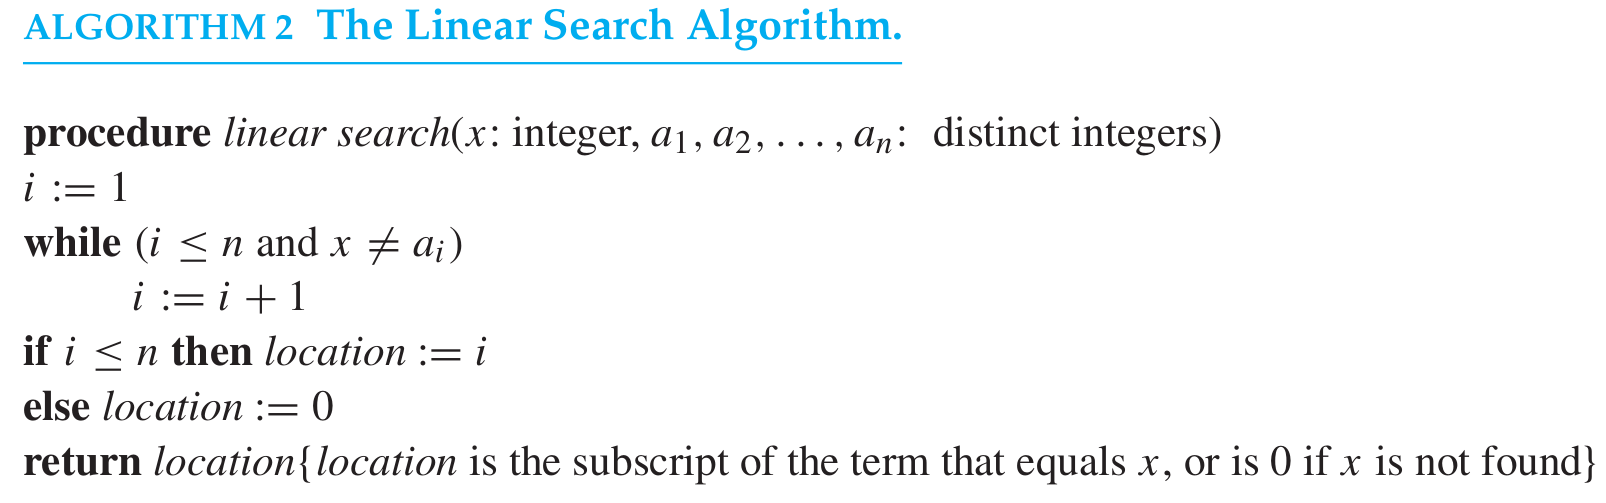
\includegraphics[width=\textwidth]{linear-search}
\end{center}
\end{frame}

\begin{frame}{Getum við gert betur?}
\begin{itemize}
 \item Línuleg leit virkar oft ágætlega
 \begin{itemize}
  \item Hún er einföld
  \item Virkar á allar runur
 \end{itemize}
 \item Ef við vitum meira um rununa getum við oft notað öflugri aðferðir
 \item Ef runan er röðuð getum við notað helmingunarleit
\end{itemize}
\end{frame}

\begin{frame}{Röðuð runa}
\begin{tcolorbox}[title=Röðuð runa]
Runa $a_1, \ldots, a_n$ er stranglega vaxandi sé $a_1 < a_2 < \ldots < a_n$.

Runa $a_1, \ldots, a_n$ er stranglega lækkandi sé $a_1 > a_2 > \ldots > a_n$.

Runa sem er stranglega vaxandi eða stranglega lækkandi er röðuð.
\end{tcolorbox}

Oft er gert ráð fyrir að röðuð runa sé vaxandi.
\end{frame}



\begin{frame}{Næst}
Reiknirit (kafli 3.1) og vöxtur falla (kafli 3.2)
\end{frame}


\end{document}
